\documentclass{article}

% if you need to pass options to natbib, use, e.g.:
%     \PassOptionsToPackage{numbers, compress}{natbib}
% before loading tackling_climate_workshop_style

% ready for submission
% \usepackage{tackling_climate_workshop_style}

% to compile a preprint version, e.g., for submission to arXiv, add add the
% [preprint] option:
%     \usepackage[preprint]{tackling_climate_workshop_style}

% to compile a camera-ready version, add the [final] option, e.g.:
%     \usepackage[final]{tackling_climate_workshop_style}

% to avoid loading the natbib package, add option nonatbib:
     \usepackage[nonatbib]{tackling_climate_workshop_style}

\usepackage[utf8]{inputenc} % allow utf-8 input
\usepackage[T1]{fontenc}    % use 8-bit T1 fonts
\usepackage{hyperref}       % hyperlinks
\usepackage{url}            % simple URL typesetting
\usepackage{booktabs}       % professional-quality tables
\usepackage{amsfonts}       % blackboard math symbols
\usepackage{nicefrac}       % compact symbols for 1/2, etc.
\usepackage{microtype}      % microtypography
\usepackage{amsmath}
\usepackage{graphicx}
\usepackage{gensymb}
\usepackage{subfigure}
% \usepackage{subcaption}


\title{An Inversion Algorithm of Ice Thickness and InSAR Data for
the State of Friction at the Base of the Greenland Ice Sheet}

% The \author macro works with any number of authors. There are two commands
% used to separate the names and addresses of multiple authors: \And and \AND.
%
% Using \And between authors leaves it to LaTeX to determine where to break the
% lines. Using \AND forces a line break at that point. So, if LaTeX puts 3 of 4
% authors names on the first line, and the last on the second line, try using
% \AND instead of \And before the third author name.

\author{%
  David S.~Hippocampus\thanks{Use footnote for providing further information
    about author (webpage, alternative address)---\emph{not} for acknowledging
    funding agencies.} \\
  Department of Computer Science\\
  Cranberry-Lemon University\\
  Pittsburgh, PA 15213 \\
  \texttt{hippo@cs.cranberry-lemon.edu} \\
  % examples of more authors
   \And
   Coauthor \\
   Affiliation \\
   Address \\
   \texttt{email} \\
   \AND
   Coauthor \\
   Affiliation \\
   Address \\
   \texttt{email} \\
  % \And
  % Coauthor \\
  % Affiliation \\
  % Address \\
  % \texttt{email} \\
  % \And
  % Coauthor \\
  % Affiliation \\
  % Address \\
  % \texttt{email} \\
}

\begin{document}

\maketitle

\begin{abstract}
With the advent of climate change and global warming, the Greenland Ice Sheet (GrIS) has been melting at an alarming rate, losing over 215 Gt per yr, and accounting for 10\% of mean global sea level rise since the 1990s. It is imperative to understand what dynamics are causing ice loss and influencing ice flow in order to successfully project mass changes of ice sheets and associated sea level rise. This work applies machine learning, ice thickness data, and horizontal ice velocity measurements from satellite radar data to quantify the magnitudes and distributions of the basal traction forces that are holding the GrIS back from flowing into the ocean. Our approach uses a hybrid model: InSAR velocity data trains a linear regression model, and these model coefficients are fed into a geophysical algorithm to estimate basal tractions that capture relationships between the ice motion and physical variables. Results indicate promising model performance and reveal significant presence of large basal traction forces around the coastline of the GrIS.

%The results of this work pave the way towards a new method of associating ice loss with sea level changes.%
% Our algorithm extracts relevant features including the $\varepsilon_{xx}$, $\varepsilon_{yy}$, and $\varepsilon_{xy}$ components of the viscous responses caused by forces on the ice, trains a linear regression model to predict ice velocities, and uses these model coefficients to quantify forces and distributions of basal tractions across the GrIs. 

\end{abstract}

\section{Introduction}

With the advent of climate change and global warming, ice sheets worldwide have been melting at an alarming rate. The rate of ice mass loss has increased sixfold from 81 billion tons in the 1990’s to 475 billion tons in the 2010s \cite{the_imbie_team_mass_2020}. The largest contributor to global ice loss is the Greenland Ice Sheet (GrIS), losing over 215 Gt of ice per yr, and accounting for 10\% of mean global sea level rise since the 1990s ~\cite{stocker_climate_2013}. Rising sea levels have a wide array of disastrous impacts, including coastal erosion, storm surges, flooding, spread of disease, and habitat loss that will only continue to worsen in a warming climate \cite{pattyn_greenland_2018}. It is imperative to understand what dynamics are influencing ice loss and ice flow in order to successfully project mass changes of the GrIS and associated sea level rise.

Recent advances in satellite remote sensing systems have produced high-resolution maps of the Earth, making them an ideal tool for studying motion across large ice sheets. Two-pass Interferometric Synthetic Aperture Radar (InSAR) satellites use radar observations from multiple trips over an area of interest to determine surface motion \cite{wild_differential_2019}. In this work, we utilize high-resolution InSAR ice velocity measurements of the GrIS derived from satellite imagery captured by the ESA's Sentinel-1 fleet \cite{nagler_sentinel-1_2015}. By inverting the data using a linear regression model, we quantify previously poorly-characterized forces and distributions of basal tractions that are holding the GrIS back from flowing into the ocean. Initial results reveal significant presence of large basal tractions forces around the coastline of the ice sheet.

\section{Previous Work}

Glaciologists have traditionally classified ice motion as a viscous flow \cite{morland_steady_1980}. This motivated prior researchers at Stony Brook University to use bedrock and ice elevations of the GrIS, derived from topographical data provided by the NOAA's ETOPO1 dataset, to map a vertically integrated gravitational potential energy (GPE) of the GrIS \cite{information_ncei_etopo1_nodate}. The primary focus of the research was capturing a relationship between GPE and the velocity of viscous ice flow, and thus the researchers assumed that the ice was moving along a frictionless base. However, the GPE velocity calculations vastly overestimated the ground truth InSAR ice velocities. This difference reinforces the notion that the basal tractions between the ice and the bedrock have a major influence over ice motion and ice velocity \cite{maier_basal_2021}. However, these forces have been poorly characterized as they remain buried beneath thousands of meters of ice \cite{maier_basal_2021}. Our work extends prior research to bridge the discrepancies between the GPE and InSAR ice velocities caused by the basal tractions, providing us a deeper understanding of the dynamics of the forces holding the GrIS back from flowing into the ocean. By employing machine learning and regression to perform an inversion, we are able to use InSAR and GPE velocity data to infer basal tractions that could not have been directly observed. Our novel approach uses a hybrid model: our velocity data is used to train a linear regression model, and these model coefficients can be fed into a geophysical algorithm to estimate distributions of basal traction forces that capture relationships between the ice motion and physical variables. To our knowledge, this is the first AI-driven work separating GPE and basal traction forces to understand ice sheet dynamics.

% After achieving a proper fit, the model coefficients would be able to provide valuable insight to the distributions of basal tractions, and could also be translated to view the strain rates across the GrIs.%

\section{Methods}

\subsubsection{Dataset}
Our data comes from two sources: ETOPO1 and Sentinel-1 radar satellite imagery. ETOPO1 provides topographical ice and bedrock elevation measurements which are used to calculate the thickness of the ice, and then generate gravitational potential energies (GPE) across the entire ice sheet \cite{information_ncei_etopo1_nodate}. Roughly 1800 Sentinel-1 scenes were used with InSAR feature tracking techniques to derive surface horizontal ice velocity measurements of the GrIS \cite{nagler_sentinel-1_2015}. Both global-level datasets were parsed using the geopandas library to focus on the GrIS from 2016-2017 \cite{jordahl_geopandasgeopandas_2020}. 

%Our data vector is also a model too, as it involves the velocity field of the InSAR associated with our GPE model, which predicts very high as the GPE values are four orders higher than the InSAR values.%

%Our d vector is almost a negative GPE value, which is why our linear regression coefficents are so high.%

\subsubsection{Inversion Set Up}

Our inversion equation is given by:

$$
\vec{d}=\overline{\overline{G}} m=v_{\text {InSAR}}-v_{GPE}
$$

$\vec{d}$ is our velocity field representing the difference between the InSAR and GPE velocities. To create our design matrix, $\overline{\overline{G}}$, we partitioned the GrIS into 1000 grid cells (each with size 2° x 2°) and generated 3 basis functions ($\varepsilon_{xx}$ - Horizontal East and West effective body forces, $\varepsilon_{yy}$ - Horizontal North and South effective body-forces, and $\varepsilon_{xy}$ - Shear effective body-forces) representing the ice's viscous thin-sheet responses for each cell. $m$ is our linear-regression inversion model. Our goal to find best linear combination $\overline{\overline{G}} m$ that predicts $\vec{d}$.

%Our original experiments used 40 grid cells (each 10° x 10°), and we noticed considerable performance improvements increasing the resolution of our G matrix.%

\subsubsection{Model}

This is a linear inversion task, where the effective body-forces in one grid cell can have effects on its surrounding cells and beyond. Thus, it requires a regression model. We use Least Squares Regression from the sklearn library, which has shown to perform well in inversion tasks \cite{lines_review_1984}. To further generalize and optimize the fit of our model, we also employed Ridge (Tikhonov) and LASSO regularization methods, with loss functions defined as $|| \overline{\overline{G}} m-\vec{d}\left\|_{2}+a^{2}\right\| m \|_{1}$ and $|| \overline{\overline{G}} m-\vec{d}\left\|_{2}+a^{2}\right\| m \|_{2}^{2}$ respectively \cite{marquardt_ridge_1975, tibshirani_regression_2011}. We used the trade-off (L-curve) criterion to determine our optimal smoothing parameter, shown in Figure \ref{Fig:Data1c} along with its performance metrics.

\begin{figure}[!htb]
   \begin{minipage}{0.33\textwidth}
     \centering
     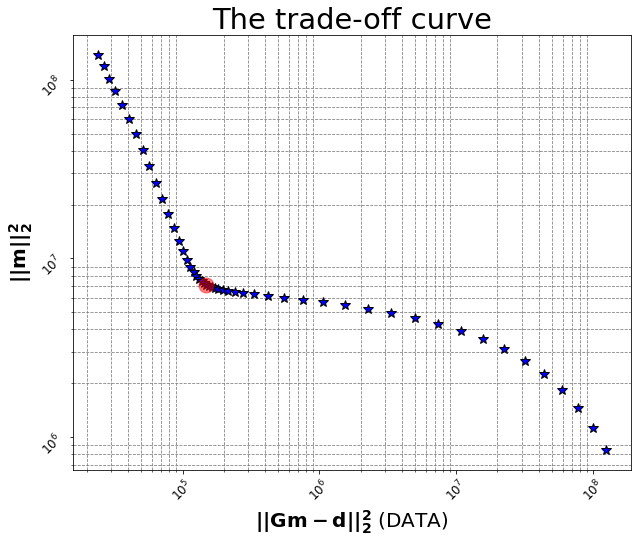
\includegraphics[width=.925\linewidth]{figures/Ridge_Trade_Off_USING.png}
     \caption{Ridge trade-off curve}\label{Fig:Data1a}
    %  \subfloat[1a]
   \end{minipage}\hfill
   \begin{minipage}{0.33\textwidth}
     \centering
     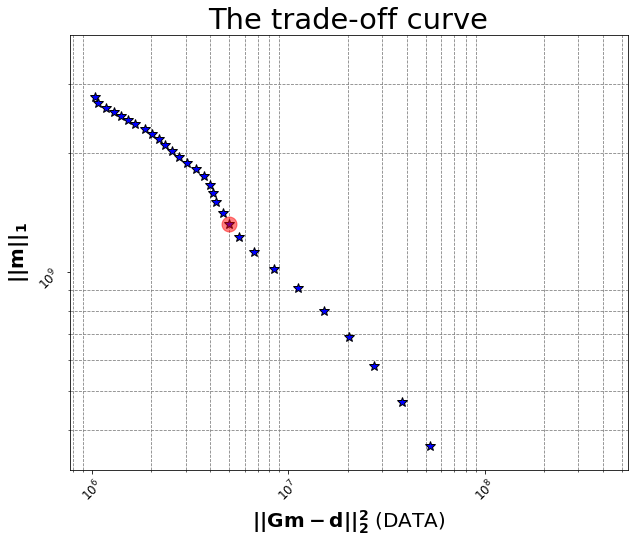
\includegraphics[width=.925\linewidth]{figures/LASSO_Trade_Off_100_Zoomed_In_USING.png}
    %  \subfloat[1b]
     \caption{LASSO trade-off curve}\label{Fig:Data1b}
   \end{minipage}
   \begin{minipage}{0.33\textwidth}
    \centering
     \begin{tabular}{l|l|l}
        \textbf{Metric} & \textbf{Ridge} & \textbf{LASSO} \\
        \hline
        Best $\alpha$ & 0.1520 & 0.0324 \\
        R$^{2}$ & \textbf{0.9994} & 0.9852 \\
        RMSE & \textbf{6.3651} & 27.6796 \\
        MAE & \textbf{4.3038} & 24.3230 \\
    \end{tabular}
    % \subfloat[1c]
    \caption{Smoothing params and performance metrics}\label{Fig:Data1c}
  \end{minipage}
\end{figure}

\section{Results}

Both the Ridge and LASSO regression models achieved a near identical fit to the velocity field, achieving $R^{2}$ values of 0.999 and 0.985 respectively. The Ridge model predictions (green vectors) have been plotted against the ground truth velocity field (red vectors) in Figure \ref{Fig:Data4}, highlighting the accuracy of the predictions. Given the unusually high $R^{2}$ score, we are planning on testing this model on larger datasets to verify this accuracy. We can now take the model's coefficients and convert our strain rate basis functions from $\overline{\overline{G}}$ to basal tractions through the geophysical algorithm described in Finzel et al. \cite{finzel_surface_2015}. The Ridge basal traction predictions are plotted in Figure \ref{Fig:Data5}, and indicate that the largest basal tractions responsible for holding the GrIS together lie on the coastline of the ice sheet.

%6 lines long

\begin{figure}[!htb]
   \begin{minipage}{0.48\textwidth}
     \centering
     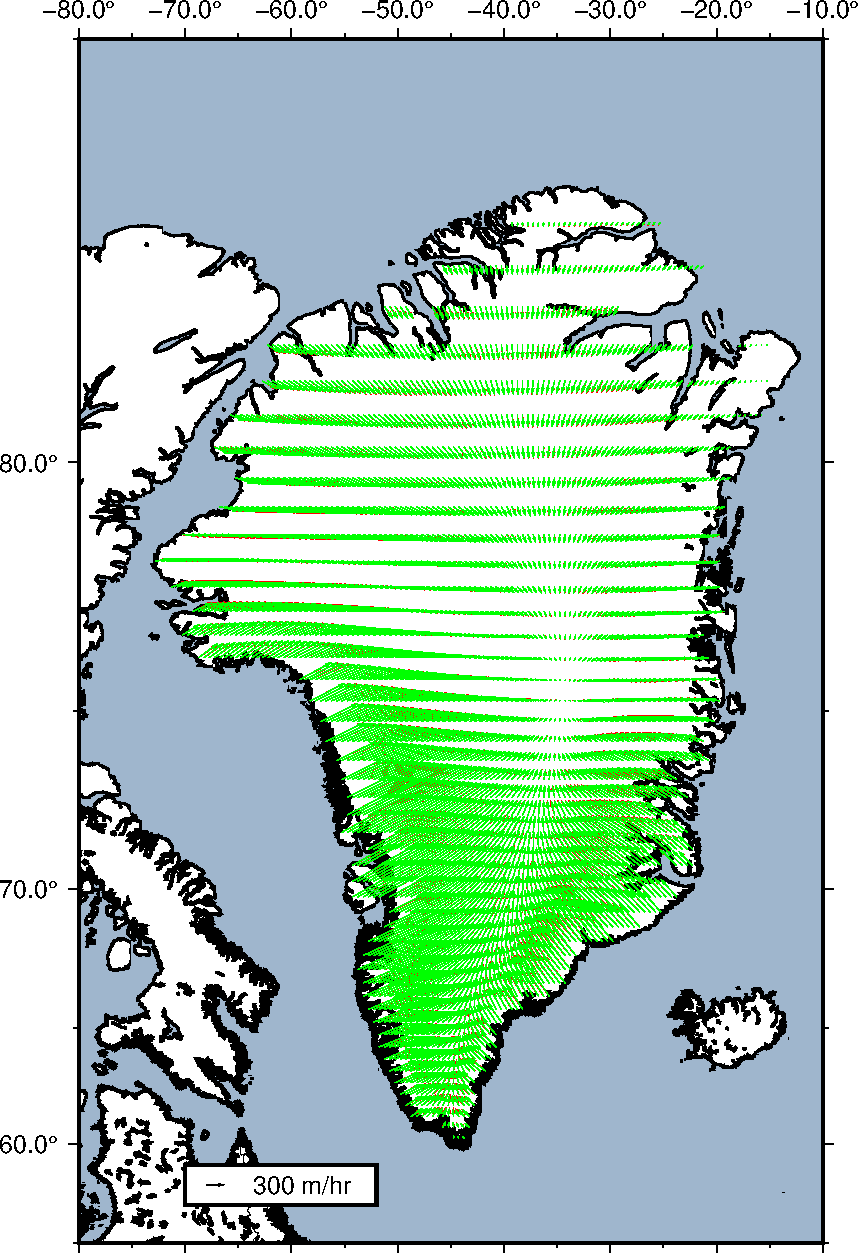
\includegraphics[width=.7\linewidth]{Ridge_pred_REAL.pdf}
     \caption{Ridge Model Velocity Predictions}\label{Fig:Data4}
   \end{minipage}\hfill
   \begin{minipage}{0.48\textwidth}
     \centering
     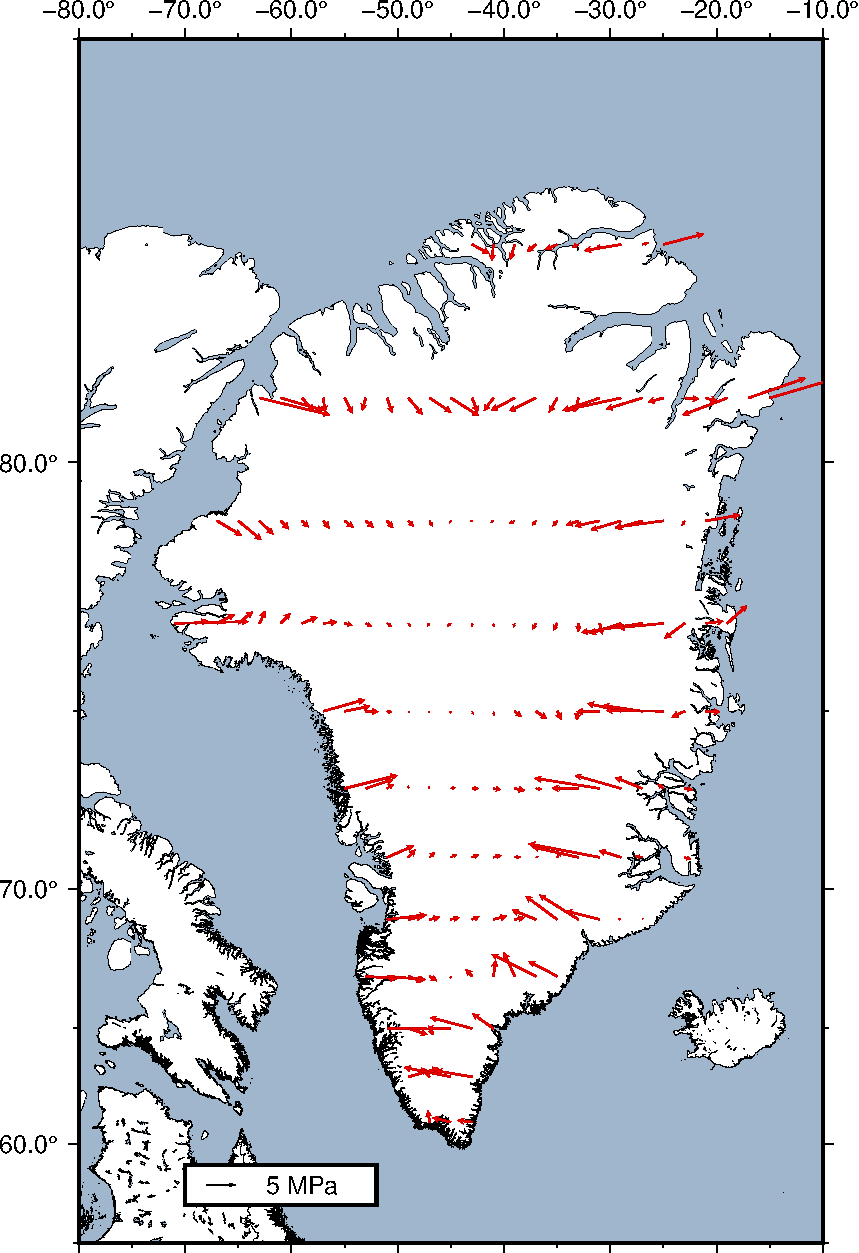
\includegraphics[width=.7\linewidth]{figures/greenland_traction_Ridge_0.15199.pdf}
     \caption{Ridge Basal Traction Predictions}\label{Fig:Data5}
   \end{minipage}
\end{figure}

\section{Conclusion and Future Work}

In this work, we developed an inversion algorithm for quantifying the magnitudes and distributions of basal tractions of the Greenland Ice Sheet. This is achieved via a hybrid approach, where our velocity data trains a linear regression model, and these model coefficients are fed into a geophysical algorithm to estimate basal tractions. This work has large implications on the ability to quantify basal tractions and how they are keeping the GrIS together, and serves as a step towards modeling ice loss and flux in relation to seawater intrusion, friction, and other forces. In the future, we hope to make this model more accurate and generalizable to other ice sheets so that it can become a helpful tool for climate scientists modelling rising sea levels. Our approach demonstrates the promise of applying AI to gain a deeper understanding of ice sheets, giving us valuable insight towards rising sea levels needed to stop climate change.

% Our approach to further optimize the fit of this model, we hope to explore the application of deep learning to improve the fit of this model, and use this work to closely monitor rising sea levels of the GrIS and beyond.
%We are currently looking for more data spanning more time or also for the Antarctic Ice Sheet.%
%REMEMBER TO CTRL F FOR BLANK AT THE END%
\bibliography{references}
\bibliographystyle{ieee_fullname}

\end{document}